\title{}
\author{}
% Remove command to get current date
\date{}
%% Based on a TeXnicCenter-Template by Tino Weinkauf.
%%%%%%%%%%%%%%%%%%%%%%%%%%%%%%%%%%%%%%%%%%%%%%%%%%%%%%%%%%%%%

%%%%%%%%%%%%%%%%%%%%%%%%%%%%%%%%%%%%%%%%%%%%%%%%%%%%%%%%%%%%%
%% HEADER
%%%%%%%%%%%%%%%%%%%%%%%%%%%%%%%%%%%%%%%%%%%%%%%%%%%%%%%%%%%%%
\documentclass[a4paper,twoside,10pt]{report}
% Alternative Options:
%	Paper Size: a4paper / a5paper / b5paper / letterpaper / legalpaper / executivepaper
% Duplex: oneside / twoside
% Base Font Size: 10pt / 11pt / 12pt


%% Language %%%%%%%%%%%%%%%%%%%%%%%%%%%%%%%%%%%%%%%%%%%%%%%%%
\usepackage[USenglish]{babel} %francais, polish, spanish, ...
\usepackage[T1]{fontenc}
\usepackage[ansinew]{inputenc}

\usepackage{lmodern} %Type1-font for non-english texts and characters


%% Packages for Graphics & Figures %%%%%%%%%%%%%%%%%%%%%%%%%%
\usepackage{graphicx} %%For loading graphic files
%\usepackage{subfig} %%Subfigures inside a figure
%\usepackage{tikz} %%Generate vector graphics from within LaTeX

%% Please note:
%% Images can be included using \includegraphics{filename}
%% resp. using the dialog in the Insert menu.
%%
%% The mode "LaTeX => PDF" allows the following formats:
%%   .jpg  .png  .pdf  .mps
%%
%% The modes "LaTeX => DVI", "LaTeX => PS" und "LaTeX => PS => PDF"
%% allow the following formats:
%%   .eps  .ps  .bmp  .pict  .pntg


%% Math Packages %%%%%%%%%%%%%%%%%%%%%%%%%%%%%%%%%%%%%%%%%%%%
\usepackage{amsmath}
\usepackage{amsthm}
\usepackage{amsfonts}


%% Line Spacing %%%%%%%%%%%%%%%%%%%%%%%%%%%%%%%%%%%%%%%%%%%%%
%\usepackage{setspace}
%\singlespacing        %% 1-spacing (default)
%\onehalfspacing       %% 1,5-spacing
%\doublespacing        %% 2-spacing


%% Other Packages %%%%%%%%%%%%%%%%%%%%%%%%%%%%%%%%%%%%%%%%%%%
%\usepackage{a4wide} %%Smaller margins = more text per page.
%\usepackage{fancyhdr} %%Fancy headings
%\usepackage{longtable} %%For tables, that exceed one page


%%%%%%%%%%%%%%%%%%%%%%%%%%%%%%%%%%%%%%%%%%%%%%%%%%%%%%%%%%%%%
%% Remarks
%%%%%%%%%%%%%%%%%%%%%%%%%%%%%%%%%%%%%%%%%%%%%%%%%%%%%%%%%%%%%
%
% TODO:
% 1. Edit the used packages and their options (see above).
% 2. If you want, add a BibTeX-File to the project
%    (e.g., 'literature.bib').
% 3. Happy TeXing!
%
%%%%%%%%%%%%%%%%%%%%%%%%%%%%%%%%%%%%%%%%%%%%%%%%%%%%%%%%%%%%%

%%%%%%%%%%%%%%%%%%%%%%%%%%%%%%%%%%%%%%%%%%%%%%%%%%%%%%%%%%%%%
%% Options / Modifications
%%%%%%%%%%%%%%%%%%%%%%%%%%%%%%%%%%%%%%%%%%%%%%%%%%%%%%%%%%%%%

%\input{options} %You need a file 'options.tex' for this
%% ==> TeXnicCenter supplies some possible option files
%% ==> with its templates (File | New from Template...).



%%%%%%%%%%%%%%%%%%%%%%%%%%%%%%%%%%%%%%%%%%%%%%%%%%%%%%%%%%%%%
%% DOCUMENT
%%%%%%%%%%%%%%%%%%%%%%%%%%%%%%%%%%%%%%%%%%%%%%%%%%%%%%%%%%%%%
\begin{document}

\pagestyle{empty} %No headings for the first pages.


%% Title Page %%%%%%%%%%%%%%%%%%%%%%%%%%%%%%%%%%%%%%%%%%%%%%%
%% ==> Write your text here or include other files.

%% The simple version:
\title{General tiling in a finite container}
\author{Shahar Tal}
%\date{} %%If commented, the current date is used.
\maketitle

%% The nice version:
%\input{titlepage} %%You need a file 'titlepage.tex' for this.
%% ==> TeXnicCenter supplies a possible titlepage file
%% ==> with its templates (File | New from Template...).


%% Inhaltsverzeichnis %%%%%%%%%%%%%%%%%%%%%%%%%%%%%%%%%%%%%%%
\tableofcontents %Table of contents
\cleardoublepage %The first chapter should start on an odd page.

\pagestyle{plain} %Now display headings: headings / fancy / ...



%% Chapters %%%%%%%%%%%%%%%%%%%%%%%%%%%%%%%%%%%%%%%%%%%%%%%%%
%% ==> Write your text here or include other files.

%\input{intro} %You need a file 'intro.tex' for this.


%%%%%%%%%%%%%%%%%%%%%%%%%%%%%%%%%%%%%%%%%%%%%%%%%%%%%%%%%%%%%
%% ==> Some hints are following:

\chapter{Motivation}\label{Motivation}

The problem we want to solve is how to arrange the pieces in tiling puzzles, from the “put together” type. The innovation is that there is no more coupling to the specific kind of the puzzle. Once we have a mapping (which we will define later) as part of the input, the search can be done in general way.
\\
\\
The puzzle types which are used as proof of concept are based on a grid lattice: squares/ cubes (2-d/ 3-d), spheres and hexagonal prism. The lattice of squares is the best known of these puzzle types and has many implementations. The sphere lattice is much more complicated and the hexagonal prism lattice provides an example where not all the transformations are symmetric (rotating hexagonal prism from z-grid to x is forbidden). Here are some grids from the above families and a solution for each one of them.
\\
\\
fig1-grid examples.jpg 1.1
\\
\begin{figure}[p]
	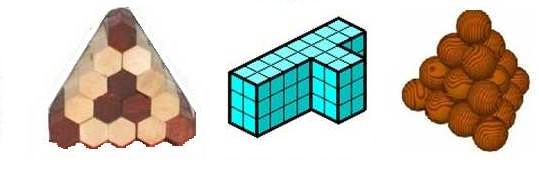
\includegraphics[width=12mm]{fig1-grid_examples.jpg}
	\caption{Grid examples}
	\label{fig:Grid examples}
\end{figure}
\\
fig2-example for solution.jpg 1.2

\begin{figure}[p]
	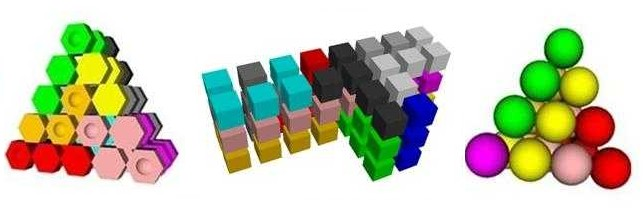
\includegraphics[width=12mm]{fig2-example_for_solution.jpg}
	\caption{example for solution}
	\label{fig:example for solution}
\end{figure}

\chapter{Presentation}\label{Presentation}

As mentioned before, the core is based on the mapping, the presentation. The grid and the pieces are represented as a graph and sub-graphs of this graph. The nodes present the atoms – the smallest piece: a cube 1x1x1, a sphere or a hexagonal prism. The directed edges present the connection between atom and its neighbor (plus the opposite connection – always in pairs: North & South, etc). For example: in a square, it’s North, South, East and West (and in cube also back and front); in a sphere there are 6 neighbors around it, 3 above and 3 below, for total of 12 neighbors. Once the presentation exists all we need is to embed (to place) the forest of the pieces on the grid graph.
\\
\\
Here is a 2-d squares grid, the pieces and one of the possible solutions:
\\
\\
fig3-test case.jpg 2.1
\\
\begin{figure}[p]
	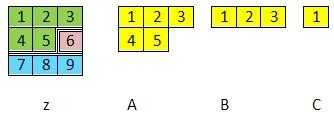
\includegraphics[width=12mm]{fig3-test_case.jpg}
	\caption{Test case}
	\label{fig:Test case}
\end{figure}

\\
\\
The placement in the example is: piece A is on atoms 1-5 of the grid; piece B on 7-8, and C on the 6.  A part of the edge placement is: in piece B, the East/ West edge between atoms 1 and 2 is placed on identical edges on the grid, but between atoms 7 and 8. The solution can be treated (grid type independent) as the list of the grid atoms: A1 A2 A3 A4 A5 C1 B1 B2 B3, or by the pieces order and their orientation in the solution: A1 C1 B1, where the 1 stands for the first orientation from all the existing.
\\
\\
The placement is only in the nodes hierarchy, as the edges between different pieces are not placed explicitly. The placement of two adjacent pieces connects them by the appropriate edges in the grid.
\\
\\
An example for an edge without explicit placement: in the grid, on the edge North/South in z3-6 lies the edge North/South from A3 to C1, which are different pieces.
\\
\\
Beside the definition of the edges types, we define the possible transformations on an atom. The result of this is the set of pieces’ orientations. For example: in a square you can rotate from x-axis to y (let’s call it XY transformation) in clockwise. And also reflection (using any direction in 2-d) – the vertical reflection is the same as flipping it around the z=0 plane. A cube has three axises so there are three kinds of transformations: XY, XZ, and YZ. In a hexagonal prism, you can rotate every atom by 60 degrees, and reflect it in inverse (the front side switches with the back one).
\\
\\
Transformation is in fact a function t from edge to edge. In the first example t(North) = West, t(East) = North, t(South) = East, t(West) = South. Applying it on all the atoms in a piece, makes the transformation on the whole piece. The above t is equivalent to clock-wise rotate, by 90 degrees.
\\
\\
As the problem is placement, we can call it “exact cover”, known to be a hard problem. Each algorithm will try all the possibilities. The improvements will be in reducing the “trial and error” steps of placement tries. The scope for placements is the result of all the orientations of all the pieces (and the grid by itself).
\\
\\
No need to say that a piece placement is successful if it does not go out from the grid, or overrides another piece.
\\
\\
For example, in the left 2-D squares grid, all the 8 orientations are in the right. In the first row there are all the clock-wise rotations, and in the second, on each rotation, its vertical reflection.
\\
\\
fig4-7 in "Implied", total-8.jpg 2.2
\\
\begin{figure}[p]
	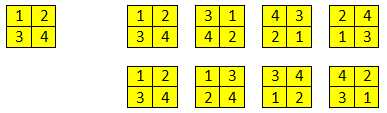
\includegraphics[width=12mm]{fig4-7_in_implied,_total-_8.jpg}
	\caption{7 in Implied, total 8}
	\label{fig:7 in Implied, total 8}
\end{figure}

\\
\\As opposed to that, in this grid there is no symmetry in x-axis and y-axis, so there are only 4 orientations.
\\
\\
fig5-3 in "Implied", total-4.jpg 2.3
\\
\begin{figure}[p]
	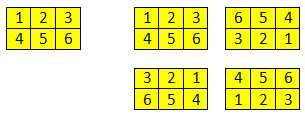
\includegraphics[width=12mm]{fig5-3_in_implied,_total-_4.jpg}
	\caption{3 in Implied, total 4}
	\label{fig:3 in Implied, total 4}
\end{figure}

\\
The orientations amount influences the extra existing solutions for each unique solution. Meaning, the total amount of solutions in the second example is maximum four times (depending on the pieces) the unique solutions amount, unless we request to find them all without distinguishing the unique solutions.
\\
\\
For example, in 2x2 squares grid, if the pieces were the above mentioned C, and a new additional piece shaped like L, we would have one unique solution, plus 3 more, for a total of 4. Despite the 8 orientations of the grid, the L piece has only 4, so it determines the total solutions amount.
\\
\\
Each piece (including the grid) induces on its atoms an ordering relation. For example, the ids order is by the y-coordinate and then x, or: the advance is by rows (from top to bottom) and in each one, by columns (from left to right), like the atoms numbers in the above examples.

\chapter{Method}\label{Method}

Before we describe the algorithm, let’s sketch the core idea and the required initial stages, essential for the execution. The rest of the initial stages, are used to improve the number of legal piece placement.
\\\\
The first algorithm, the trivial one, is brute-force and depth-first. It places piece by piece, by the atom order in the grid. In each piece, all the orientations are tried. After each placement, it advances (by the given order relation) to the next atom in the grid, which is not already occupied. Once the entire grid has been placed, a success is going to be written and the solution is added to the output set. Now, in order to find more legal placements (solution), it back tracks: It removes the last placed piece and goes further, for the next permutation (the next orientation of the last removed piece, or the next piece in queue). It should be noted that the test (= the entire grid that has been placed) is not on the pieces, as there are problems where there are more pieces than necessary (and the user needs to find the redundant).
\\
\\
For example:
\\
\\
fig6-test case, empty solution.jpg 3.1
\\
\begin{figure}[p]
	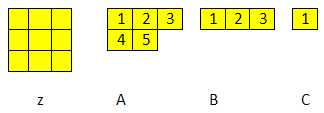
\includegraphics[width=12mm]{fig6-test_case,_empty_solution.jpg}
	\caption{Empty grid}
	\label{fig:Empty grid}
\end{figure}
\\
Piece A has 8 orientations, B has 2 (as the layout is symmetric horizontally), and C has only 1. The number of permutations (potential placements/ solutions) is 1x2x8 multiply by the number of options to order the pieces – the factorial of 3. In each one of the 96 options we stop immediately as we find out that it is an impossible placement, for example: in the above orientations, placing B and then C and A is impossible.
\\
\\
Again, the search is after the unique solutions, without repetitions because of symmetries. The algorithms deal with search only after these solutions. From there it finds instantaneously the rest.

\chapter{Initialization}\label{Initialization}

\subsubsection{Possible Orientations}

Find all the possible orientations by automatically compute the number of available transformation in each kind of transformation. For example, in a cube, there are four transformations of the type XY (and the same for XZ and YZ). Assuming each kind of transformation repeats itself after some invocations (t**n(edge) = edge, for each edge) one can find all the orientations of a piece by performing all kind of possible transformations, one after another. For example, in a 3-d piece, there is a need to generate the 4x4x4=64 orientations, and remove repetitions. This is a na?ve way, based on no information on the piece attributes (in the 3-d grid, d=3, we have in fact only dx2d=24 possible orientations, imagining reflection to the 4-d, 48).\\\\
The first algorithm, the trivial one, is brute-force and depth-first. It places piece by piece, by the atom order in the grid. In each piece, all the orientations are tried. After each placement, it advances (by the given order relation) to the next atom in the grid, which is not already occupied. Once the entire grid has been placed, a success is going to be written and the solution is added to the output set. Now, in order to find more legal placements (solution), it back tracks: It removes the last placed piece and goes further, for the next permutation (the next orientation of the last removed piece, or the next piece in queue). It should be noted that the test (= the entire grid that has been placed) is not on the pieces, as there are problems where there are more pieces than necessary (and the user needs to find the redundant).
\\
\\
o	Automatically compute the number of possible orientations in each kind, performed by applying the transformation over and over again until the returning to the source. This is the above 4.
\\
\\
o	Remove repetitions, performed by comparing DFS scanning of the current orientation to the previous orientations. DFS scans are equal if the order of the scan is the same in both orientations, with no relevance to the ids.
\\
\\
fig7-comparing by DFS.jpg 4.1
\\
\begin{figure}[p]
	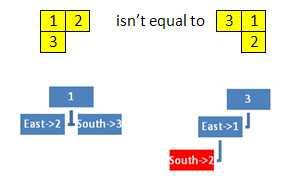
\includegraphics[width=12mm]{fig7-comparing_by_DFS.jpg}
	\caption{Comparing by DFS}
	\label{fig:Comparing by DFS}
\end{figure}

Here, we go South from the root, vs. go there after an East edge.
\\
\\
Note:  the entry points (two trees) for the DFS, the roots, can be all the possible ones: All atoms from the current orientations, versus all atoms from all of the previous orientations. This is because we can compare the above B piece to its vertical reflection (3>2>1 vs. 1>2>3) and only in such way can we conclude they are the same (when we compared root 3 vs. root 1).
\\
\\
The remove repetitions stage has an exception, the unique piece. It will come later.
\\\\
\subsubsection{Unique and Implied}

Mapping unique solution to its implied solutions (the symmetries) - relevant only if the request is a search after the unique solutions only (the default).
\\
\\
o	Decision on the unique piece – made by finding the one with the maximum number of orientations. If there are a few pieces like that, choose arbitrarily.
\\
\\
For example, in the above grid, the unique is A.
\\
\\
o	Generate all the possible orientation of the grid. In each orientation, remove the corresponding orientation from the unique’s orientation.
\\
\\
For example, both the grid and the piece A have 8 orientations. We remove all of them, beside the given one (in this specific case, A must be placed in the grid with the same given orientation).
\\
\\
o	“Implied” array – as mentioned before, the “compare by DFS scanning” marks each node (when it meets the node in the first time). It is used as bread crumb - to identify we were there before. The mark is the id of the current atom of the piece we compare with. In the beginning, right after the user defines the pieces, this id is the index of the atom in the atoms list. Only after this, the id changes to be according to the order relation. So, when duplicity was found in the previous stage, an entry will be created in the implied array, which contains these marks according to the order in which the DFS scanned the piece. That, of course, if this entry is unique.
\\
\\
For example, the above 2x2 squares grid can be treated as 1-d array which contains 1 2 3 4. The implied entries are 4 3 2 1, 3 1 4 2 and so on.
\\
\\
o	“Unique in implied” – For each orientation of the unique piece, find in which symmetric it is placed in the same orientation, as it is in the unique solution that was found. This will allow us to filter duplicate solution, as explained later.
\\
\\
For example, one of the unique solutions for the 5x4x3 squares grid and pentominoes pieces is – floor by floor
\\\\
fig8-unique in the found solution.jpg 4.2
\\
\begin{figure}[p]
	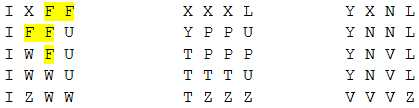
\includegraphics[width=12mm]{fig8-unique_in_the_found_solution.jpg}
	\caption{Unique in the found solution}
	\label{fig:Unique in the found solution}
\end{figure}
\\
\\In the 6th implied solution (from 7) – total of 8 symmetries per unique solution – the unique piece F was placed in the same orientation exactly. In order to get this implied solution, reflect the floor, swap the first and last floors.
\\\\
fig9-unique in one of the "Implied".jpg 4.3
\\
\begin{figure}[p]
	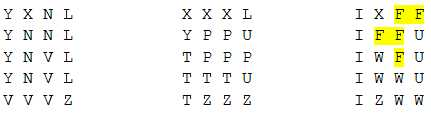
\includegraphics[width=12mm]{fig9-unique_in_one_of_the_Implied.jpg}
	\caption{Unique in one of the Implied}
	\label{fig:Unique in one of the Implied}
\end{figure}
\\\

\chapter{The algorithm – second look}\label{The algorithm – second look}

In every found solution, there is a check if it is a duplicate one, which appeared before in the same presentation (A1 C1 B1) or as an identical permutation (if there are M identical pieces, there will be M! duplicate solutions). If a duplicate was found, we skip on this solution. Identical solution is possible if the unique piece was placed at an implied solution in a specific location (atom index) and in other solution, also at the same location. In such case, the solution that we found will be saved in the solutions list with potential for duplicates. When the current piece for placement is the unique, we check where it will be placed in the implied solution (using the implied array and the “unique In Implied” described before), and allow only one of those to be considered as a unique solution. This can be done arbitrarily, by requiring that the location in the current try is less than the location in the implied solution. As a result, the search for duplicates does not go over all the list of solutions every time, but on a fraction of it (we can search for hash values of the solution, like CRC of “A1C1B1”).
\\
\\
Another way to check duplicates is by blocking the implied location of the unique piece once a solution was found. Here, the check will be in the “trial and error” step (when placing the unique piece) and not at the end of it (potential solution was found) – not comparing a whole solution but only locations.

\chapter{Results}\label{Results}

\subsubsection{Implementation}

The method of presentation was implemented in two engines (for total of 5,500 lines of code). The first engine is the described algorithm, the trivial one. When running on 5x4x3 squares grid with pentominoes pieces, on a dual core 2.2 GHz computer with Sun’s Java Virtual Machine 6, it takes about 3 days. For that reason, an option to save the current state of execution was added (to stop the process and continue it later). In addition, the two engines include simple parallelism for use with the modern multi core computers.\\
\\
•	Saving the current state – the recursive method transported to be iterative, then saving the stack content.
\\
\\•	Simple parallelism – splitting the search tree, but only on the first piece to be placed. For example, if the pieces are 1...n and the split is for two parallel threads, in the first placement of the first thread, the piece will be with index 1...n/2, and in the second thread, the piece will be in the second half.
\\\\
\subsubsection{A brief on Dancing Links}

The second engine – the dancing links algorithm known as DLX – is based on an open source implementation by Apache taken from its Hadoop project. The described presentation was added as a layer over the engine, to make it appropriate for the problem. This engine makes significant improvement and based on a paper by Knuth.
\\\\
In short, we solve here an NP complete problem – exact cover. In the input a 0/1 matrix is given and the search is after the set of rows in which there is a single 1 in every column. This is the placement. The input is received by relating the columns as an atom in the grid (covered atom = 1). We add extra columns to the input, new one per piece. In these columns there is a 1 in the corresponding id (this time it is the index) of the piece which makes the placement. The rows are all the possible places of every piece in its different orientations.
\\\\For example, the above placement is the following set of rows, out of all the existing rows:
\\\\
1 1 1 1 1 0 0 0 0 A 1 0 0
\\
0 0 0 0 0 0 1 1 1 B 0 1 0
\\
0 0 0 0 0 1 0 0 0 C 0 0 1
\\\\
In the whole set of rows, the piece C is listed 9 times (as this is the number of the atoms in the grid), piece B can be vertical or horizontal, so it is listed 6 times (3 rows + 3 columns), and so on with piece A.
\\\\
The algorithm is based on the trivial, except there’s a different implementation for the heap. Instead of using pointers (as in regular recursive calls) it uses array. When back-tracking, we removed a change from the state, by “next [previous [x]] <-- next[x]” (the same with previous). Now “undo” can be done easily, by “next [previous [x]] <-- x”, which is the “dance” step. Using this trick, improves dramatically the performance. In addition, each recursive call “chooses” the smallest sub-tree (the Size heuristic) by finding the column with the minimum amount of 1s.
\\\\
\subsubsection{Improvements}

After some sort of improvements (some attached) the time in the trivial engine decreased to 40 minutes, and in the DLX – to 40 seconds. The improvements include, beside regular usage of performance profiler, tries to reduce the amount of “trial and error” placements.
\\\\
•	Anchor atom calculation – Calculated automatically according to the order relation on the grid. In the above example these are A1, B1, and C1. This allows the try to place a piece to begin with the correct atom. Actually, it improves performance by 45\%, theoretically, by 40\%. For example, in a piece with 5 atoms, in average, in half of the cases we’ll start with the anchor atom, in comparison to computing it in advance. 1/(5/2) = 40\%.
\\\\o	Mark grid ids – induce the atoms order to compute the id by DFS. In each step (passing an edge) of the DFS it updates the id according to the edge mark.
\\\\For example, if we relate an id to an atom according to its vertical distance from the axises center (+/-10 in South/ North) and then its horizontal distance (+/-1 in East/ West) we will receive a two-digit number: yx.
\\\\o	Find the first atom in this order: the smallest one.
\\In the example, it’s always the most left atom in the top row.
\\\\•	Remove impossible – for each atom of the grid, and each piece and orientation, check if a placement is possible, and save it in a look-up-table. It improves performance by up to 50\% (usually there is no option to place all the orientation of a piece on the boundaries, so the more the grid is, the better performance gain achieved, as the boundaries atoms have smallest percent from all the grid atoms. In addition, remove orientation which has no option to place (because the size of grid, like the above piece A on a 2x2 grid).
\\\\•	Island size – before a placement trial, compute the current island (the empty area which can be placed). If it is smallest than the current smallest un-placed piece (in a sense of atoms amount) back-track. Improvement: 35\%.
\\\\o	Computing the island size – as in the DFS, but here the placement is inverted. Continue count the free atoms as long as the current one is atom.\\
\\•	Trips calculation – Save the DFS paths. The scan is recursive, and also check for each atom if we where there. To reduce the overhead involved in naive DFS, the order of the visits is saved, aka from where (atom and piece) and on which edge.
For example, in the above A piece, assuming the order of the edges is East, West, South and North, the result of the DFS  is: from atom 1 go EAST (to atom 2), from atom 2 East (to atom 3), from 2 go SOUTH (to 4), and from 4 WEST (to 5).
\\

\begin{tabular}{|c|c|c|}
\hline Level & Trivial (Iterative/ Recursive) & DLX (with S size heuristic \\
\hline 3 & 3,833 & 1,790 \\
\hline 4 & 15,459 & 9,250 \\
\hline 5 & 60,412 & 33,156 \\
\hline 6 & 212,484 & 87,987 \\
\hline 7 & 609,062 & 191,095 \\
\hline 8 & 1,287,453 & 340,362 \\
\hline 9 & 1,908,405 & 431,556 \\
\hline 10 & 1,581,423 & 309,800 \\
\hline 11 & 120,498 & 68,082 \\
\hline 12 & 2,339 & 2,339 \\
\hline Total & 5,802,074 & 1,476,710 \\
\hline
\end{tabular}

\chapter{Resources}\label{Resources}

•	Apache. Hadoop. Hadoop is an open source Java software framework for running parallel computation on large clusters of commodity computers.
URL http://lucene.apache.org/hadoop
\\
\\
•	Donald E. Knuth. Dancing Links. In Jim Davies, Bill Roscoe, and Jim Woodcock, editors, Millennial Perspectives in Computer Science, pages 187 – 214. Palgrave, Houndmills, Basingstoke, Hampshire, 2000.
URL http://www-cs-faculty.stanford.edu/~knuth/papers/dancing-color.ps.gz


%% <== End of hints
%%%%%%%%%%%%%%%%%%%%%%%%%%%%%%%%%%%%%%%%%%%%%%%%%%%%%%%%%%%%%



%%%%%%%%%%%%%%%%%%%%%%%%%%%%%%%%%%%%%%%%%%%%%%%%%%%%%%%%%%%%%
%% BIBLIOGRAPHY AND OTHER LISTS
%%%%%%%%%%%%%%%%%%%%%%%%%%%%%%%%%%%%%%%%%%%%%%%%%%%%%%%%%%%%%
%% A small distance to the other stuff in the table of contents (toc)
\addtocontents{toc}{\protect\vspace*{\baselineskip}}

%% The Bibliography
%% ==> You need a file 'literature.bib' for this.
%% ==> You need to run BibTeX for this (Project | Properties... | Uses BibTeX)
%\addcontentsline{toc}{chapter}{Bibliography} %'Bibliography' into toc
%\nocite{*} %Even non-cited BibTeX-Entries will be shown.
%\bibliographystyle{alpha} %Style of Bibliography: plain / apalike / amsalpha / ...
%\bibliography{literature} %You need a file 'literature.bib' for this.

%% The List of Figures
\clearpage
\addcontentsline{toc}{chapter}{List of Figures}
\listoffigures

%%%%%%%%%%%%%%%%%%%%%%%%%%%%%%%%%%%%%%%%%%%%%%%%%%%%%%%%%%%%%
%% APPENDICES
%%%%%%%%%%%%%%%%%%%%%%%%%%%%%%%%%%%%%%%%%%%%%%%%%%%%%%%%%%%%%
\appendix
%% ==> Write your text here or include other files.

%\input{FileName} %You need a file 'FileName.tex' for this.


\end{document}

